\section{Analiza literatury}
\label{sec:analiza_literatury}

\subsection{Metody}
\label{sub:metody}
Big Data wymaga wyjątkowych technologii do efektywnego przetwarzania olbrzymich ilości danych w rozsądnym czasie. W 2011 roku firma {McKinsley} w swoim raporcie \cite{McKinsey2011} zaproponowała użycie do analizy Big Data takich technik jak testy A/B, crowdsourcing, eksploracja danych, algorytmy genetyczne etc.

\subsubsection{A/B testing}
\label{sub:a/b_testing}
\textbf{Testy A/B} jest to metoda badawcza służąca do wybrania lepszego rozwiązania. W założeniu osoba przeprowadzająca test posiada dwie wersje danego elementu i metrykę określającą optymalność. Aby wybrać lepsze rozwiązanie, obie wersje poddawane są temu samemu eksperymentowi. Na końcu mierzony jest wcześniej ustalony wskaźnik jakości i wybierane jest lepsze rozwiązanie \cite{paras10}.

\subsubsection{Association rule learning}
\label{sub:association_rule_learning}
\textbf{Association rule learning} jest to popularna i dobrze zbadana metoda szukania relacji pomiędzy zmiennymi w dużych bazach danych \cite{tan2005introduction}.

\subsubsection{Crowdsourcing}
\label{sub:crowdsourcing}
Termin \textbf{crowdsourcing} został po raz pierwszy zdefiniowany i użyty przez dziennikarza magazynu Wired Jeffa Howe’a \cite{Howe2006}. Odnosi się on do procesu, w którym wszelkie potrzebne moduły, serwisy, pomysły czy materiały pozyskiwane są od dużej grupy ludzi (zwłaszcza od społeczności online) w formie outsourcingu. Jest to metoda zastępująca tradycyjnych pracowników bądź dostawców. Proces ten jest często używany do podziału żmudnej pracy lub w celu pozyskiwania funduszy na finansowanie nowych firm i organizacji charytatywnych \cite{Howe2006}.

Crowdsourcing łączy wysiłki wielu wolontariuszy i pracowników tymczasowych. Każdy z uczestników wnosi do projektu niewielki nakład pracy, co przy dużej liczbie ochotników powoduje osiągnięcie określonego celu.

Crowdsourcing różni się od outsourcingu tym, że wolontariuszem może zostać każdy, a nie tylko wybrana grupa ludzi.

\subsubsection{Eksploracja danych}
\label{sub:eksploracja_danych}
\textbf{Eksploracja danych} (\textit{ang. data mining}) jest jedną z metod analizy danych. Jest to ,,nauka zajmująca się wydobywaniem informacji z dużych zbiorów danych lub baz danych'' \cite{Hand01}. Metoda ta wykorzystuje prędkość przetwarzania danych przez komputery do znalezienia prawidłowości w danych, które są zgromadzone w pewnym rodzaju bazy danych, zorganizowanej pod kątem pewnej części rzeczywistości (\textit{hurtownia danych}). 

Eksplorację danych można rozwiązać na wiele sposobów. Mogą to być:
\begin{enumerate}
    \item wizualizaje na wykresach
    \item metody statystyczne
    \item zbiory przybliżone
    \item logika rozmyta
    \item metody ewolucyjne
    \item metody uczenia maszynowego
    \item sieci neuronowe \ldots
\end{enumerate}

\subsubsection{Data Integration}
\label{sub:data_integration}
\textbf{Data fusion} i \textbf{data integration} to zbiór technik do integracji i analizy danych pochodzących z różnych źródeł \cite{lenzerini02}. Przykładowym wykorzystaniem tych technik jest połączenie danych z serwisów społecznościowych (np. Twitter, Facebook) z danymi finansowymi, aby określić stopień powodzenia kampanii reklamowej.

\subsubsection{Algorytmy genetyczne}
\label{sub:algorytmy_genetyczne}
Algorytm genetyczny jest to rodzaj algorytmu przeszukujący możliwe rozwiązania w celu znalezienia najoptymalniejszych lub najlepszych. Za ich twórcę uważa się John Henry Hollanda, który prowadził swoje badania zainspirowany ewolucją biologiczną.

Jest on zaliczany do grupy algorytmów ewolucyjnych, a więc jest jedną z technik eksploracji danych opisanej w sekcji \ref{sub:eksploracja_danych}.

Poniższy schemat blokowy przedstawia zasadę działania tego algorytmu:
\begin{figure}[h]
    \centerline{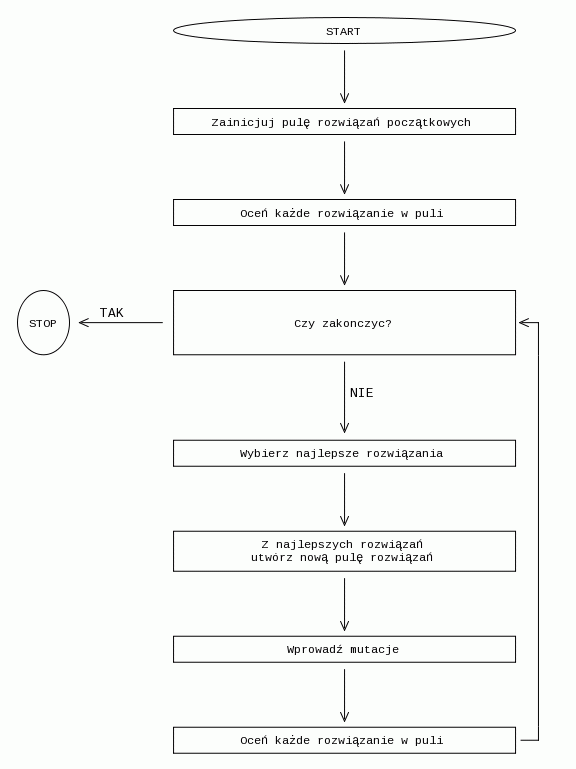
\includegraphics[scale=0.5]{obrazki/algorytm_genetyczny.png}}
    \caption{Schemat działania algorytmu genetycznego}
    \label{fig:alg_gen}
\end{figure}

\subsubsection{Uczenie maszynowe}
\label{sub:uczenie_maszynowe}
\textbf{Uczenie maszynowe} to dziedzina informatyki mocno powiązana ze sztuczną inteligencją. Uczenie maszynowe zajmuje się projektowaniem i konstrukcją algorytmów i systemów, których potrafią się ucyzć (zdobywać wiedzę) z uzyskanych danych.

Algorytmy uczenia maszynowego można podzielić na dwa rodzaje: nadzorowane i nienadzorowane. Algorytmy nadzorowane na wejściu dostają wzorcowy zbiór danych, który służy im za bazę do oceny bądź klasyfikacji nowych danych. Algorytmy nienadzorowane nie mają takiego zestawu danych. Przykładem algorytmu nienadzorowanego jest algorytm \textit{k-means} \cite{sugar03}.

\subsubsection{Przetwarzanie języków naturalnych}
\label{sub:nlp}
\textbf{Przetwarzanie języków naturalnych} (\textit{NLP -- Natural Language Processing}) jest przykładowym wykorzystaniem uczenia maszynowego i wiedzy z zakresu lingwistyki. Jest to zbiór technik służących do analizy języków naturalnych -- czyli takich, jakimi posługują się ludzie na co dzień. Jednym z bardziej znanych zastosowań tych algorytmów jest analiza sentymentów postów na Twitterze \cite{agarwal11}. Dane pochodzące z Twittera były też używane do estymowania aktywności wirusa świńskiej grypy H1N1 \cite{signorini11}.

\subsubsection{MapReduce}
\label{sub:mapreduce}
\textbf{MapReduce} jest to platforma stworzona przez pracowników firmy Google.  W 2004 r. dwóch z nich (Jeffrey Dean oraz Sanjay Ghemawat) wydali artykuł \cite{dean08}, w którym przedstawili nowy system. 

System ten ma za zadanie tworzenie aplikacji działających jednocześnie na tysiącach komputerów. Jak nazwa wskazuje, mamy w nim doczynienia z dwoma częściami obliczeń, a mianowicie mapowaniem (map) oraz redukcją (reduce).

Największym plusem tego podejścia jest możliwość łatwego rozdzielenia operacji na różne serwery, ponieważ można założyć, że każda operacja mapowania jest niezależna od pozostałych.

\subsubsection{Statystyka}
\label{sub:statystyka}
\textbf{Statystyka} jest nauką matematyczną zajmującą się zbieranem, organizjacją, analizą i interpretacją, a także prezentacją danych \cite{statystyka:podrecznik}. Metody statystyczne są często używane do znajdywania i określania związków w zestawach danych. Przykładem metody statystycznej są testy A/B opisane w sekcji \ref{sub:a/b_testing}.

\subsubsection{Przetwarzanie sygnałów}
\label{sub:przetwarzanie_sygnalow}
\textbf{Przetwarzanie sygnałów} jest nauką zajmującą się analizą i interpretacją sygnałów, analogowych bądź cyfrowych \cite{smith97}, takich jak sygnału radiowe, audio, czy obrazki.

\subsubsection{Symulacja}
\label{sub:symulacja}
,,\textbf{Symulacja} to technika służąca do imitowania działania całego systemu lub też tylko naśladowania pewnej sytuacji (ekonomicznej, militarnej, mechanicznej, etc.) poprzez użycie odpowiednich modeli lub urządzeń w celu zdobycia informacji, czy też w celach dydaktycznych'' \cite{www:symulacja}.

Technika symulacji jest najpopularniejsza tam, gdzie analityczne dojście do rozwiązania byłoby niemożliwe, lub prowadziłoby do dużych nakładów finansowych lub czasowych.

Symulacje \textit{Monte-Carlo} są klasą algorytmów symulacji, polegającą na wykonywaniu tysięcy symulacji z różnymi, losowymi parametrami, aby uzyskać histogram rozkładu prawdopodobieństwa \cite{math:monte-carlo}.

Do przeprowadzania symulacji komputerowej stosuje się narzędzia takie jak SciLab \cite{www:scilab}, język programowania GPSS \cite{www:gpss} oraz @Risk \cite{www:risk}.

\subsubsection{Szereg czasowy}
\label{sub:szereg_czasowy}
\textbf{Szereg czasowy} to ciąg obserwacji pewnego zjawiska w kolejnych jednostlach czasu. Analiza szeregów czasowych uzywa technik mających źródła w statystyce, jak i w przetwarzaniu sygnałów.

\subsubsection{Wizualizacja}
\label{sub:wizualizacja}
Techniki \textbf{wizualizacji} naukowej są używane do tworzenia obrazków, diagramów, wykresów bądź animacji, których zadaniem jest ułatwienie zrozumienia i przekzazanie pewnych wniosków wynikających z analizy danych \cite{lawrence1994}. Do tworzenia prostych wykresów i diagramów często używa się takiego oprogramowania jak R \cite{www:R} bądź Octave \cite{www:octave}.

\subsection{Implementacje}
% TODO

\subsection{Big Data wg Google}
\label{ssub:google}
System Big Data Google'a składa się z kilku elementów, m.in. rozproszonego systemu plików, bazy danych NoSQL, architektury MapReduce.

\subsubsection{GFS}
\label{ssub:gfs}
\textbf{GFS} (\textit{Google File System}) jest rozproszonym systemem plików uzywanym przez Google'a na swoich serwerach, opisanym w \cite{ghemawat03}. GFS jest zoptymalizowany do przechowywania olbrzymich ilości danych, generowanych przez usługi Google'a, głównie wyszukiwarkę. W przeciwieństwie do większości systemów plików, GFS nie jest zaimplementowany w jądrze systemu, tylko jako zwyczajna biblioteka.

W klastrze GFS występują dwa typy serwerów:
\begin{itemize}
    \item \textbf{Master} -- tylko jeden w danym systemie
    \item \textbf{Chunk Server} -- może ich być wiele
\end{itemize}
Każdy plik w systemie jest dzielony na bloki (wielkości 64MB), identyfikowane64-bitowym kluczem. Bloki te są przechowywane na \textit{Chunk Server}ach. Każdy taki blok jest replikowany kilka razy w klastrze.
Serwer \textit{Master} nie przechowuje samych bloków, lecz tylko metadane z nimi związane, takie jak mapowanie kluczy na lokacje bloków i ich kopii, jakie bloki składają się na jakie pliki, etc.
Dostęp do danych działa w następujący sposób:
\begin{enumerate}
    \item Aplikacja pyta serwera \textit{Master} o lokację żądanego bloku
    \item Jeśli na danym bloku nie są przeprowadzane żadne operacje, \textit{Master} zwraca adres do bloku
    \item Aplikacja modyfikuje dane bezpośrednio na \textit{Chunk server}ze wskazanym przez adres podanym przez serwer główny.
\end{enumerate}

Przykładowa infrastruktura klastra GFS ukazana jest na obrazku \ref{fig:google:gfs}.

\begin{figure}
    \centering
    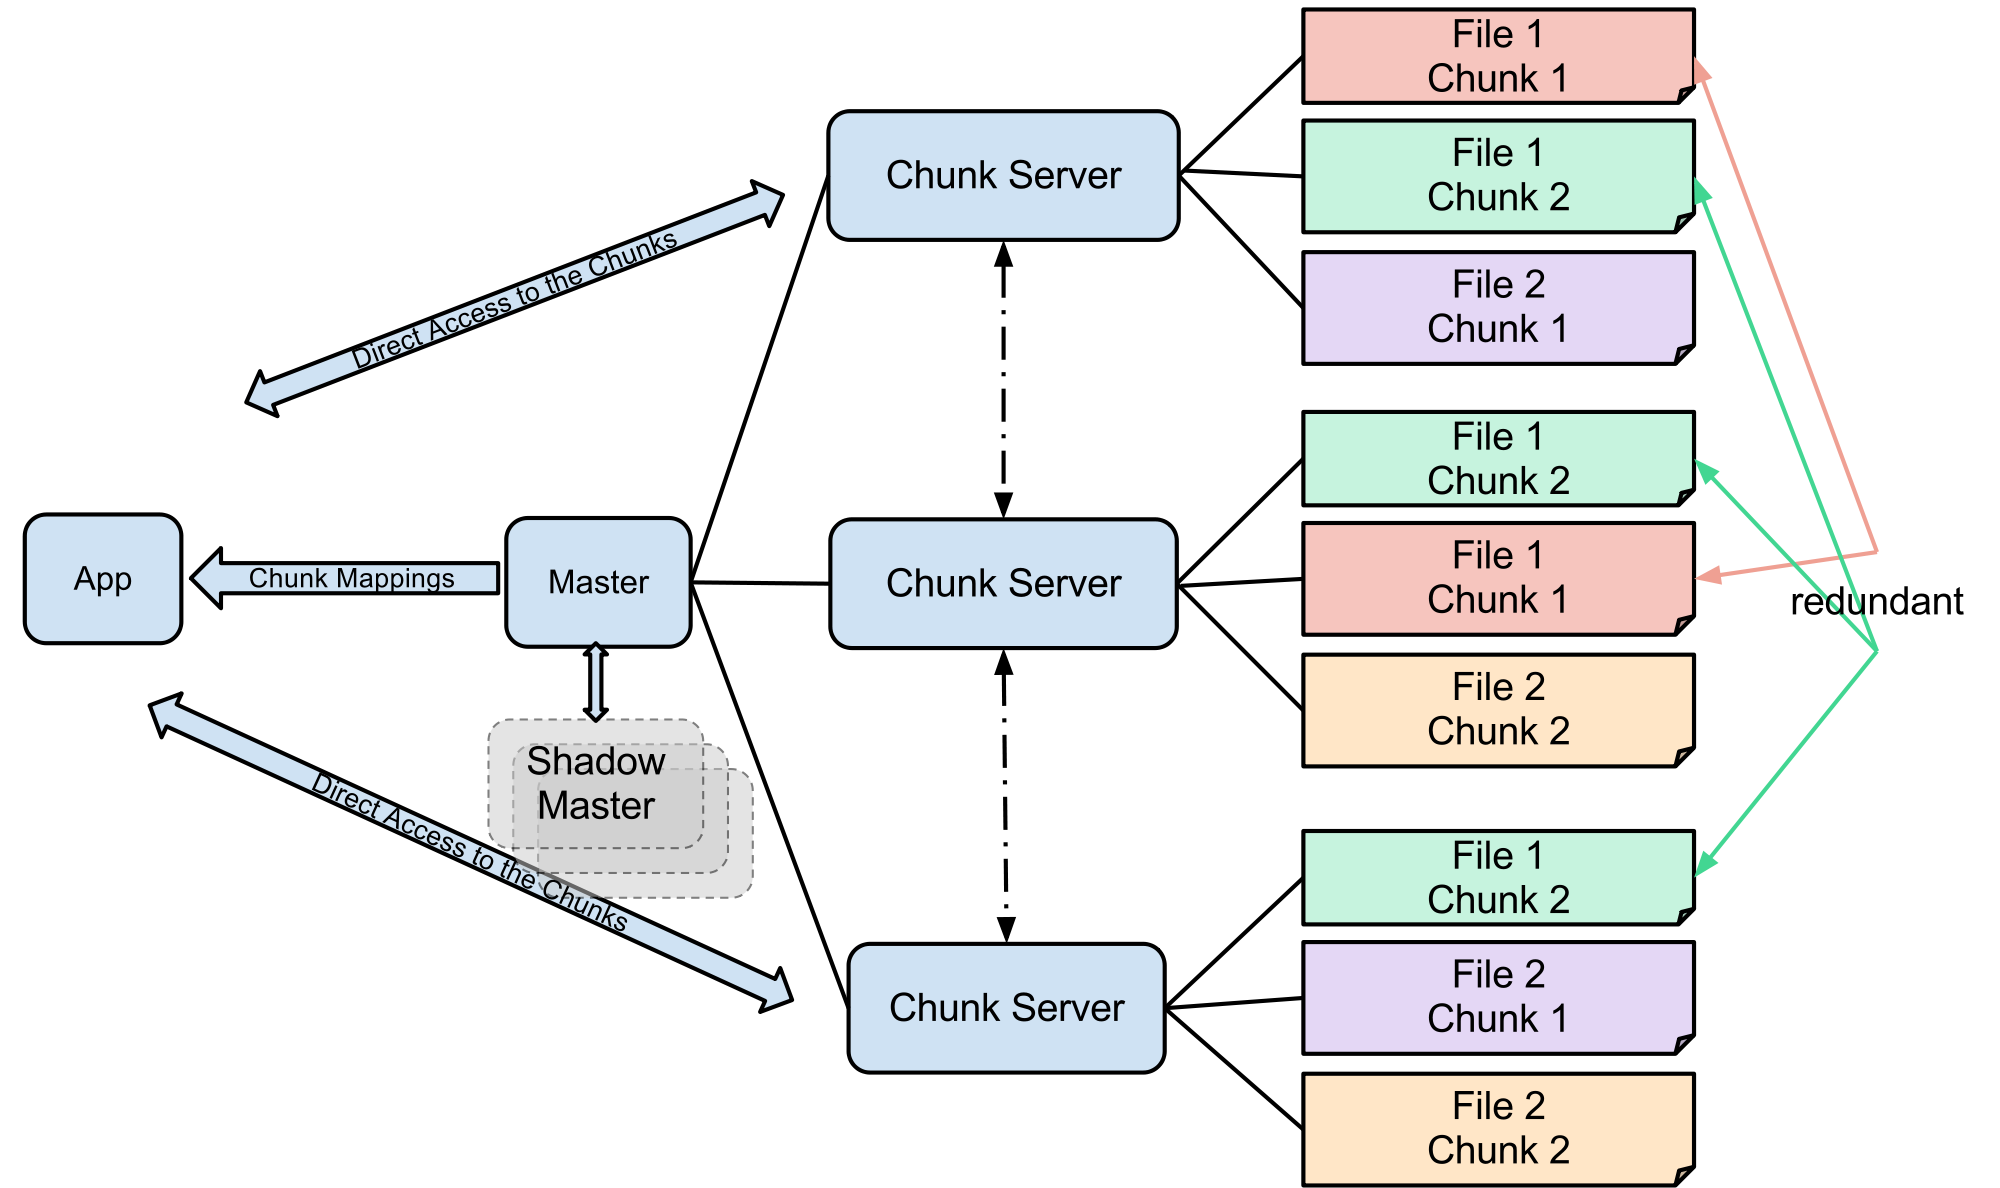
\includegraphics[scale=0.2]{obrazki/GoogleFileSystemGFS.png}
    \caption{Google File System -- infrastruktura}
    \label{fig:google:gfs}
\end{figure}

\subsubsection{BigTable}
\label{ssub:bigtable}
\textbf{BigTable} jest bazą danych NoSQL używaną przez Google. 

BigTable jest rzadką, rozproszoną mapą, indeksowaną za pomocą dwóch ciągów znakowych (wiersza i kolumny) oraz 64-bitowej daty. Każda wartość w mapie jest po prostu tablicą bajtów
$$(row: \texttt{string} \times column: \texttt{string} \times timestamp: \texttt{int64}) \mapsto \texttt{string}$$
Tabelki BigTable są optymalizowane do użytku pod GFS poprzez podział na \textit{tablety} -- segmenty tabelki podzielone wzdłuż wiersza.

Schemat struktury tabelki BigTable zaprezentowany jest na rysunku \ref{fig:google:big-table}.

\begin{figure}
    \centering
    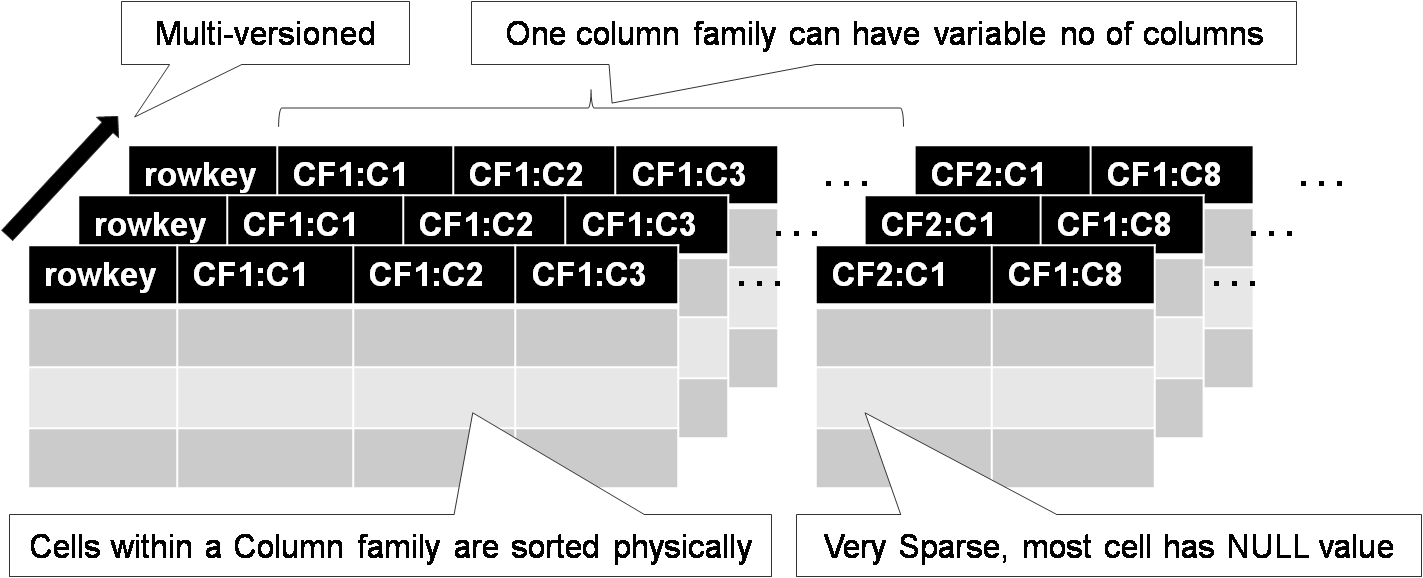
\includegraphics[scale=0.5]{obrazki/big-table.png}
    \caption{BigTable -- struktura}
    \label{fig:google:big-table}
\end{figure}

\subsubsection{MapReduce}
\label{ssub:mapreduce}
\textbf{MapReduce} jest modelem programowania, stworzonym przez Google i opisanym w \cite{dean08}. Model ten jest używany wraz z wspomnianymi wcześniej BigTable i GFS do analizy gigantycznych ilości danych w Google.

\subsubsection{BigQuery}
\label{ssub:bigquery}
Google \textbf{BigQuery} jest usługą umozliwiającą osobom trzecim skorzystanie z infrastruktury Google do analizy Big Data \cite{www:google-big-query}.

\subsection{Hadoop}
\label{ssub:hadoop}
Apache Hadoop jest otwartą (open source) platformą implementującą paradygmat MapReduce \cite{dean08}, które wyprodukowało Google. Jego autorem jest Doug Cutting.

\subsubsection{Historia}
\label{ssub:hadoop_historia}
Projekt o nazwie Hadoop rozpoczęto w 2005 r. Jego tworzenie trwało stosunkowo długo, ponieważ dopiero  w 2011 r. opublikowano pierwszą wersję - Hadoop 1.0. Produkt ten od początku był tworzony jako platforma mająca na celu obsługę bardzo dużych zbiorów danych. 

\subsubsection{Ogólne działanie}
\label{ssub:ogolne_dzialanie}
Ogólną myślą Hadoop jest podzielenie dużych zbiorów danych na mniejsze, przetwarzane równolegle w węzłach wykorzystujących serwery. Wielką zaletą tej platformy jest niezależność od systemu operacyjnego oraz oczywiście wspomniana już wcześniej możliwość obsługi danych niestrukturyzowanych.

Wykorzystując narzędzia Apache Flume oraz Apache Sqoop, odpowiednio służących do wymiany danych między systemami RDBMS i Hadoop oraz przekierowanie logów systemowych do Hadoop w czasie rzeczywistym, możliwe jest zintegrowanie już stworzonego systemu razem z platformą Hadoop. Zaletą tego podejścia jest możliwość pracy z danymi niezależnie od ich wielkości. Wraz z powiększeniem się ilości danych należy tylko dodać nowe węzły Hadoop oraz serwery, które przetwarzają dane.

\subsubsection{Apache Hadoop}
\label{ssub:apache_hadoop}
Apache Hadoop jest open-sourcowym oraz skalowalnym oprogramowaniem. Jest to framework pozwalajócy na przetwarzanie bardzo dużych zbiorów danych z różnych komputerów używajóc prostego modelu programowania. Umożliwia on pracę z tysiócami obliczeniowo niezależnymi komputerami oraz petabajtami danych. Hadoop pochodzi z MapReduce oraz Google File System.

\subsubsection{Hadoop Distributed File System}
\label{ssub:hdfs}
Hadoop Distributed File System (HDFS) jest rozproszonym systemem plików zapewniajócym odporność na uszkodzenia. HDFS zapewnia dostęp o wysokiej przepustowości do danych aplikacji oraz nadaje się do obsługi aplikacji, które posiadajó duże zbiory danych. Hadoop zapewnia system plików, które mogó przechowywać dane na tysiócach serwerów i pracuje w oparciu o system MapReduce. Duże dane automatycznie dzielone só na mniejsze kawałki, które mogó być przetwarzane przez różne węzły klastra hadoop.

Obrazek \ref{fig:rozklad_danych} przedstawia rozkład danych w węzłach w czasie ładowania.

\begin{figure}[h]
    \centerline{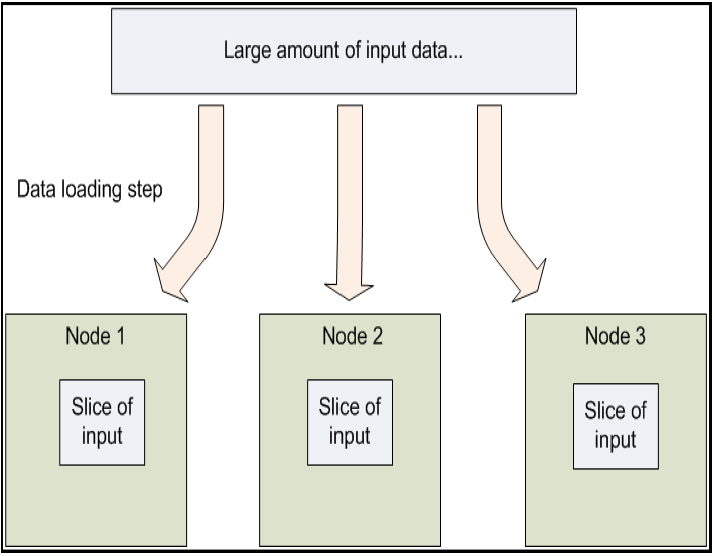
\includegraphics[scale=0.5]{obrazki/rozklad_danych.png}}
    \caption{Schemat działania algorytmu genetycznego}
    \label{fig:rozklad_danych}
\end{figure}

\subsubsection{Architektura HDFS}
\label{ssub:hdfs_architecture}
Na rysunku \ref{fig:hdfs_architecture} pokazano architekturę HDFS. Można na nim zobaczyć, że klaster HDFS składa się z pojedynczego NameNode'a (serwer główny), który odpowiedzialny jest za zarządzanie przestrzenią nazw oraz regulacją dostępności plików przez klientów. Ponadto występuje również pewna liczba DataNode'ów (węzłów danych), zwykle jeden na każdy węzeł w klastrze, które zarządzają pamięcią dołączoną do węzłów, które działają. HDFS pokazuje przestrzeń nazw systemu plików i pozwala na przechowywanie danych użytkownika w plikach. Plik podzielony jest na jeden lub więcej bloków, które przechowywane są w węzle danych. Serwer główny (NameNode) mapuje bloki do węzłów danych.
HDFS zaprojektowany jest tak, aby bardzo duże pliki przechowywane były przez maszyny w dużych klastrach. Przechowuje on  każdy plik jako ciąg bloków

\begin{figure}[h]
    \centerline{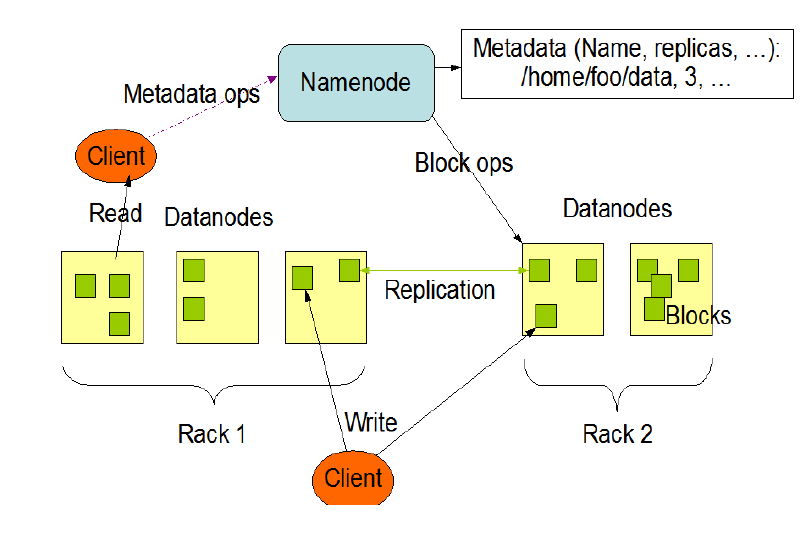
\includegraphics[scale=0.5]{obrazki/HDFS_architecture.png}}
    \caption{Architektura HDFS}
    \label{fig:hdfs_architecture}
\end{figure}

\subsubsection{Wysokkopoziomowa architektura HDFS}
\label{ssub:hdfs_high_level_architecture}
Klaster Hadoop składa się z jednego węzła ,,mistrza'' (master) i wielu węzłów ,,niewolników'' (slaves). JobTracker jest serwisem wewnątrz Hadoop, który ,,dzierżawi'' zadania MapReduce dla konkretnych węzłów w klastrze. Najlepiej jakby to były węzły, które zawierają dane, a ewentualnie są na tej samej półce.

TaskTracker jest węzłem w klastrze, który akceptuje zadania mapowania, redukcji oraz przetasowania z JobTrackera. Węzeł główny składa się z JobTrackera, TaskTrackera, NameNode'a oraz DataNode'a. Węzeł podrzędny (niewolnik) działa zarówno jako DataNode oraz TaskTracker.ś

Wszytko to zobrazowane jest na rysunku \ref{fig:hdfs_hight_level_architecture}.

\begin{figure}[h]
    \centerline{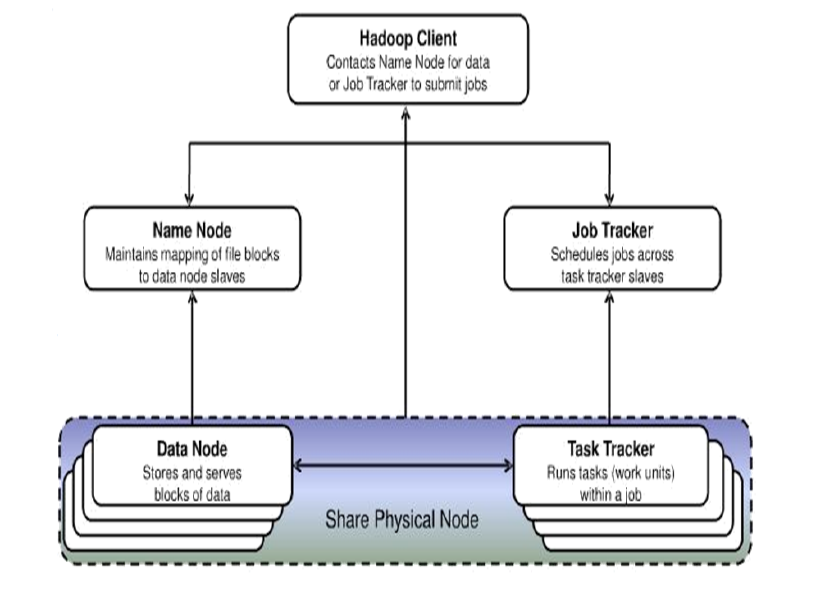
\includegraphics[scale=0.5]{obrazki/wysokopoziomowa_architektura_hadoop.png}}
    \caption{Wysokopoziomowa architektura HDFS}
    \label{fig:hdfs_hight_level_architecture}
\end{figure}


\subsubsection{Porównanie do relacyjnych baz danych}
\label{ssub:porownanie_z_relacyjnymi}
Platforma ta jest wspomagana przez stworzony przez firmę Google framework programistyczny MapReduce (opisany po krótce w sekcji \ref{sub:mapreduce}), który w znacznym stopniu ułatwia tworzenie narzędzi do analizy informacji. Jego przewagą nad relacyjnymi bazami danych jest to, że od samego początku jest przystosowany do zarządzania bazami przechowywującymi dane niestrukturalne.

Platforma Hadoop nie ma na calu zastąpienie obecną infrastrukturę baz danych, a jedynie zwiększenie efektywności zarządzania pamięcią masową oraz wszelkiego rodzaju danymi.

Większość firm korzystających z platformy Hadoop, używa je razem z relacyjnymi bazami danych. Zazwyczaj platforma ta służy do obrabiania wielkich danych, z którymi mogą sobie poradzić relacyjne bazy danych.


\subsection{Zastosowania implementacji}
\label{sub:zastosowania_implementacji}
%TODO

\subsection{Timeline}
\label{sub:timeline}
\begin{description}
    \item[styczeń 1996] \hfill \\ Larry Page i Sergey Brin z Uniwersytetu w Stanford rozpoczynają projekt badawczy dotyczący Big Data,
    \item[wrzesień 1998] \hfill \\ zostaje założona firma Google,
    \item[rok 1999] \hfill \\ Doug Cutting tworzy Lucene, kluczowy komponent Apache Nutch, Apache Solr i ElasticSearch,
    \item[rok 2000] \hfill \\ Larry Page i Sergey Brin presentują Google Design w artykule ,,The Anatomy of a Large-Scale Hypertextual Web Search Engine'',
    \item[styczeń 2001] \hfill \\ Jimmy Wales i Larry Sanger uruchamiają Wikipedię,
    \item[rok 2003] \hfill \\ Doug Cutting i Mike Cafarella tworzą i demonstrują Nutch, open-source'ową wyszukiwarkę internetową, zdolną zarządzać 100 milonami stron,
    \item[kwiecień 2004] \hfill \\ Google uruchamia Gmail
    \item[rok 2004] \hfill \\ Yonik Seeley tworzy Solr, projekt umożliwiający dodanie funkcji wyszukiwania do stron internetowych,
    \item[rok 2004] \hfill \\ Google wypuszcza artykuł o zastosowaniu metody MapReduce w Large Data Cluster,
    \item[luty 2005] \hfill \\ zostaje uruchomioty serwis YouTube,
    \item[rok 2005] \hfill \\ Doug Cutting i Mike Cafarella implementuję Hadoop[\ref{ssub:hadoop}], framework oparty o MapReduce Google'a i specyfikację GFS,
    \item[luty 2006] \hfill \\ rodzi się serwis społecznościowy Twitter,
    \item[wrzesień 2006] \hfill \\ utworzony zostaje serwis społecznościowy Facebook,
    \item[rok 2006] \hfill \\ Google prezentuje pomysł BigTable \hfill \\ skalowalny, rozporszony system przechowywania danych do zarządzania danymi strukturalnymi,
    \item[czerwiec 2007] \hfill \\ powstaje pierwsza generacja iPhone,
    \item[listopad 2007] \hfill \\ światło dzienne ujrzała pierwsza beta wersja systemu Android,
    \item[marzec 2009] \hfill \\ startuje Foursquare, serwis społecznościowy dla urządzeń mobilnych,
    \item[rok 2009] \hfill \\ Nokia Research Center rozwija Disco Project \hfill \\ lekką implementację MapReduce w języku Python,
    \item[luty 2010] \hfill \\ Shay Banon wypuszcza pierwszą wersję ElasticSearch \hfill \\ łatwo skalowalną wyszukiwarkę bazującą na Lucene,
    \item[wrzesień 2011] \hfill \\ firma BackType wypuszcza Storm \hfill \\ złożony procesor zdarzeniowy i framework do obliczeń rozproszonych,
\end{description}

\subsection{Analiza artykułów i patentów}
\label{sub:analiza_artykulow}
Analizując dane dotyczące artykułów i patentów związanych z Big Data, oraz jego różnymi implementacjami, można zauważyć, że jest to technologia rozwijająca się. Na poniżej zamieszczonych wykresach wyraźnie widać, że z roku na rok pojawia się coraz więcej artykułów, autorów, czasopism, a także patentów związanych z zagadnieniem Big Data. W przeciągu 20 lat liczba artykułów związanych z Big Data wzrosła ponad trzykrotnie, natomiast liczba autorów, którzy traktują o tym zagadnieniu w swoich publikacjach prawie czterokrotnie. Najbardziej aktywnym z pośród nich, przez ostatnie 20 lat, był J. Philippe Rushton Kanadyjski psycholog widzący zastosowanie Big Data w psychometrii. W przeciągu ostatnich 20 lat trzykotnie zwiększyła się również liczba wydawnictw, na łamach których były publikowane były teksty mające związek z Big Data, z czego najwięcej z nich pojawiło się w czasopiśmie naukowym z zakresu psychologii osobowości "Personality and Individual Differences". Dużo szybciej Big Data rozwija się, jeżeli chodzi o sprawy patentowe. Tylko w przeciągu ostatnich trzech lat liczba patentów dotyczących Big Data wzrosła ponad trzykrotnie, tak samo jak liczba instytucji je zgłaszających, z czego najwięcej zgłosiła ich Chińska firma telekomunikacyjna ZTE. Wyraźnie widać, że dziedzina Big Data cały czas jest rozwijana, oraz cieszy się coraz większym zainteresowaniem, skoro poza obecnymi już w tym obszarze "wielkimi graczami" jak chociażby Google, zaczyna się nią interesować jedna z największych firm, jednego z najszybciej rozwijających się państw na świecie.

Ponieważ zwiększa się zainterezowanie tematem Big Data, zwiększa się również zainteresowanie jego konkretnymi implementacjami, jak na przykład Hadoop, czy Map Reduce. Od czasu utworzenia tych implementacji około 8 lat temu, liczba artykułów które o nich traktowały wzrosła z zera, do ponad stu rocznie. Przyglądając się osobom, które napisały tych artykułów najwięcej, można zauważyć, że zdecydowana większość z nich jest pochodzenia chińskiego, co prawdopodobnie oznacza, że temat ten cieszy się dużym zainteresowaniem w Państwie Środka. Najwięcej artykułów znalazło się w czasopiśmie "Future Generation Computer Systems", które jest pismem branżowym o Grid, oraz eNauce. Ciekawie wygląda sytuacja związana z patentami w zakresie Hadoop, oraz MapReduce. Oczywiście bardzo łątwo jest zauważyć trend rosnący, zarówno jeżeli chodzi o ilość ilość patentów, jak i ilość instytucji je zgłaszających, jednak w 2008 roku liczba zgłoszonych patentów związanych z MapReduce była taka sama jak w roku 2012, i to za sprawą jednego tylko przedsiębiorstwa, którym jest Yahoo!. Jeżeli chodzi o Hadoop, to najwięcej patentów zgłosił uniwersytet w Nanjang, co potwierdza zainteresowanie Chińczyków tematem Big Data.

\begin{figure}
    \centering
    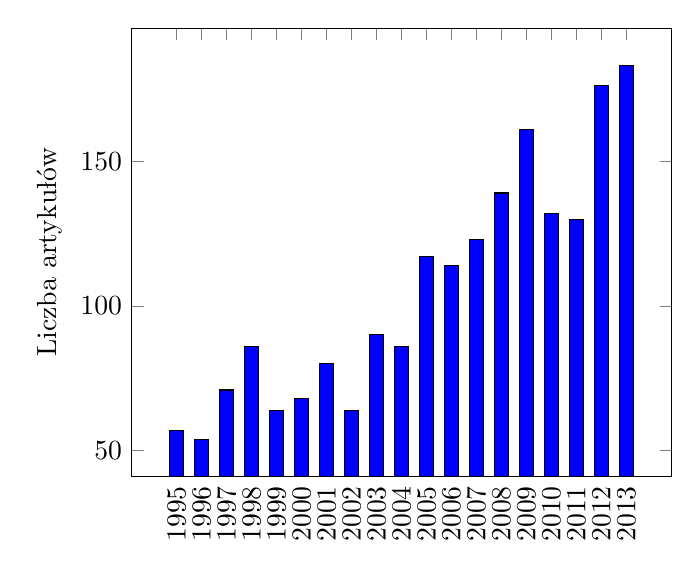
\begin{tikzpicture}
        \begin{axis}[
                bar width=5pt,
                %title=Liczba artykułów dotyczących Big Data,
                % xlabel=Rok,
                ylabel=Liczba artykułów,
                symbolic x coords={1995, 1996, 1997, 1998, 1999, 2000, 2001, 2002, 2003, 2004, 2005, 2006, 2007, 2008, 2009, 2010, 2011, 2012, 2013},
                xtick=data,
                x tick label style={rotate=90, anchor=east}
            ]
            \addplot[ybar,fill=blue] coordinates {
                (1995,   57)
                (1996,   54)
                (1997,   71)
                (1998,   86)
                (1999,   64)
                (2000,   68)
                (2001,   80)
                (2002,   64)
                (2003,   90)
                (2004,   86)
                (2005,   117)
                (2006,   114)
                (2007,   123)
                (2008,   139)
                (2009,   161)
                (2010,   132)
                (2011,   130)
                (2012,   176)
                (2013,   183)
            };
        \end{axis}
    \end{tikzpicture}
    \caption{Liczba artykułów dotyczących Big Data}
    \label{fig:art:big-data}
\end{figure}

\begin{figure}
    \centering
    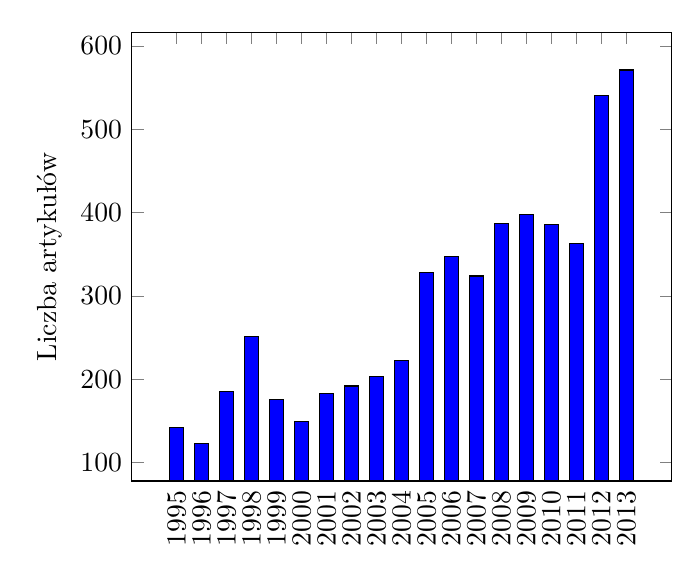
\begin{tikzpicture}
        \begin{axis}[
                bar width=5pt,
                %title=Liczba autorów piszących o Big Data,
                % xlabel=Rok,
                ylabel=Liczba artykułów,
                symbolic x coords={1995, 1996, 1997, 1998, 1999, 2000, 2001, 2002, 2003, 2004, 2005, 2006, 2007, 2008, 2009, 2010, 2011, 2012, 2013},
                xtick=data,
                x tick label style={rotate=90, anchor=east}
            ]
            \addplot[ybar,fill=blue] coordinates {
                (1995,   142)
                (1996,   123)
                (1997,   185)
                (1998,   251)
                (1999,   176)
                (2000,   150)
                (2001,   183)
                (2002,   192)
                (2003,   203)
                (2004,   223)
                (2005,   328)
                (2006,   347)
                (2007,   324)
                (2008,   387)
                (2009,   398)
                (2010,   386)
                (2011,   363)
                (2012,   540)
                (2013,   571)
            };
        \end{axis}
    \end{tikzpicture}
    \caption{Liczba autorów piszących o Big Data}
    \label{fig:aut:big-data}
\end{figure}

\begin{figure}
    \centering
    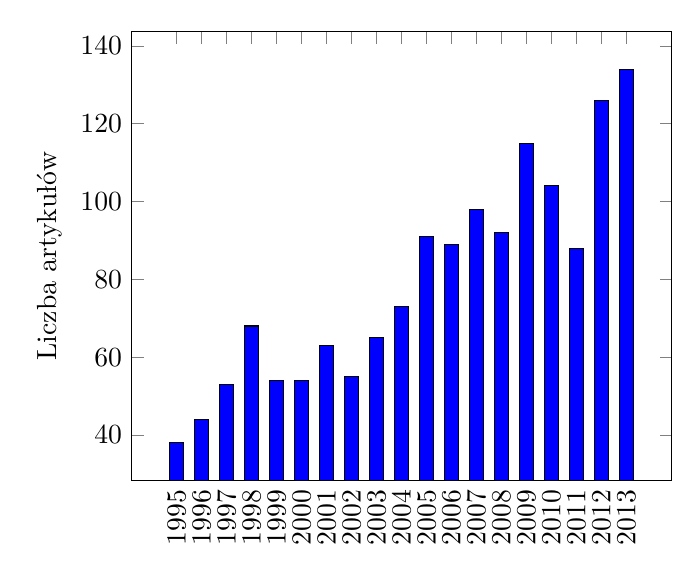
\begin{tikzpicture}
        \begin{axis}[
                bar width=5pt,
                %title=Liczba czasopism publikujących artykuły o Big Data,
                % xlabel=Rok,
                ylabel=Liczba artykułów,
                symbolic x coords={1995, 1996, 1997, 1998, 1999, 2000, 2001, 2002, 2003, 2004, 2005, 2006, 2007, 2008, 2009, 2010, 2011, 2012, 2013},
                xtick=data,
                x tick label style={rotate=90, anchor=east}
            ]
            \addplot[ybar,fill=blue] coordinates {
                (1995,   38)
                (1996,   44)
                (1997,   53)
                (1998,   68)
                (1999,   54)
                (2000,   54)
                (2001,   63)
                (2002,   55)
                (2003,   65)
                (2004,   73)
                (2005,   91)
                (2006,   89)
                (2007,   98)
                (2008,   92)
                (2009,   115)
                (2010,   104)
                (2011,   88)
                (2012,   126)
                (2013,   134)
            };
        \end{axis}
    \end{tikzpicture}
    \caption{Liczba czasopism publikujących artykuły o Big Data}
    \label{fig:journal:big-data}
\end{figure}

\begin{figure}
    \centering
    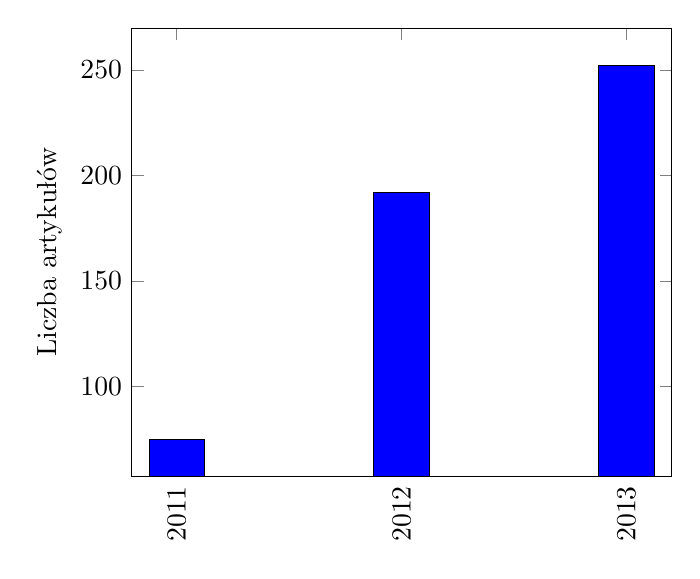
\begin{tikzpicture}
        \begin{axis}[
                bar width=20pt,
                %title=Liczba patentów dotyczących Big Data,
                % xlabel=Rok,
                ylabel=Liczba artykułów,
                symbolic x coords={2011, 2012, 2013},
                xtick=data,
                x tick label style={rotate=90, anchor=east}
            ]
            \addplot[ybar,fill=blue] coordinates {
                (2011,   75)
                (2012,   192)
                (2013,   252)
            };
        \end{axis}
    \end{tikzpicture}
    \caption{Liczba patentów dotyczących Big Data}
    \label{fig:patent:big-data}
\end{figure}

\begin{figure}
    \centering
    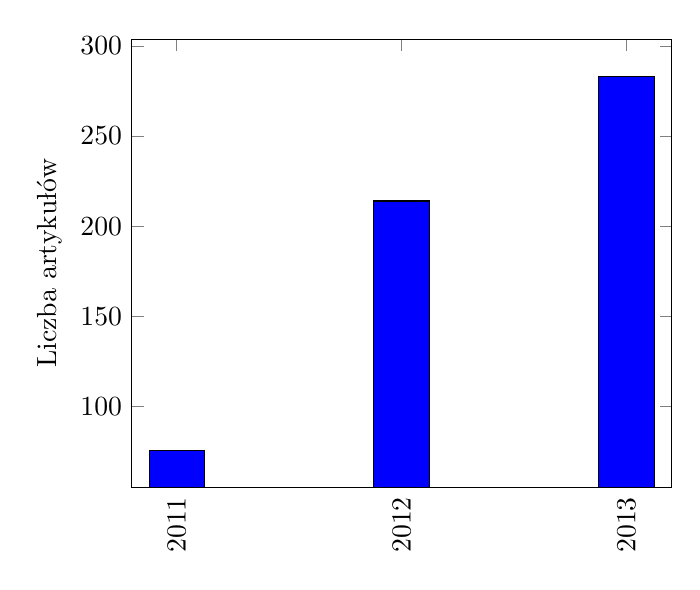
\begin{tikzpicture}
        \begin{axis}[
                bar width=20pt,
                %title=Liczba zgłaszających patenty związane z Big Data,
                % xlabel=Rok,
                ylabel=Liczba artykułów,
                symbolic x coords={2011, 2012, 2013},
                xtick=data,
                x tick label style={rotate=90, anchor=east}
            ]
            \addplot[ybar,fill=blue] coordinates {
                (2011,   76)
                (2012,   214)
                (2013,   283)
            };
        \end{axis}
    \end{tikzpicture}
    \caption{Liczba zgłaszających patenty związane z Big Data}
    \label{fig:invent:big-data}
\end{figure}

\begin{figure}
    \centering
    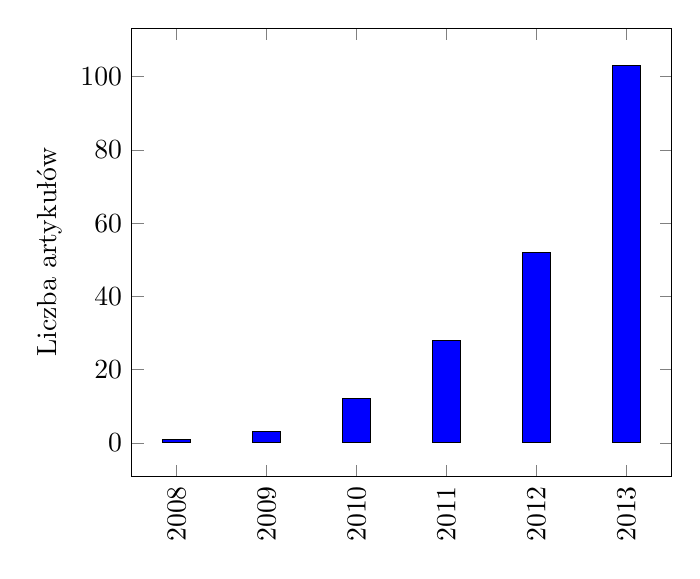
\begin{tikzpicture}
        \begin{axis}[
                bar width=10pt,
                %title=Liczba artykułów dotyczących Hadoop,
                % xlabel=Rok,
                ylabel=Liczba artykułów,
                symbolic x coords={2008, 2009, 2010, 2011, 2012, 2013},
                xtick=data,
                x tick label style={rotate=90, anchor=east}
            ]
            \addplot[ybar,fill=blue] coordinates {
                (2008,   1)
                (2009,   3)
                (2010,   12)
                (2011,   28)
                (2012,   52)
                (2013,   103)
            };
        \end{axis}
    \end{tikzpicture}
    \caption{Liczba artykułów dotyczących Hadoop}
    \label{fig:art:hadoop}
\end{figure}

\begin{figure}
    \centering
    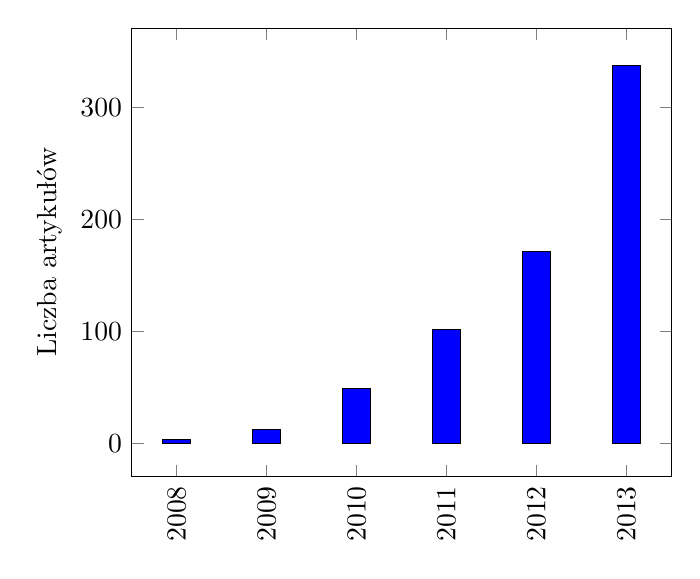
\begin{tikzpicture}
        \begin{axis}[
                bar width=10pt,
                %title=Liczba autorów piszących o Hadoop,
                % xlabel=Rok,
                ylabel=Liczba artykułów,
                symbolic x coords={2008, 2009, 2010, 2011, 2012, 2013},
                xtick=data,
                x tick label style={rotate=90, anchor=east}
            ]
            \addplot[ybar,fill=blue] coordinates {
                (2008,   4)
                (2009,   13)
                (2010,   49)
                (2011,   102)
                (2012,   171)
                (2013,   337)
            };
        \end{axis}
    \end{tikzpicture}
    \caption{Liczba autorów piszących o Hadoop}
    \label{fig:aut:hadoop}
\end{figure}

\begin{figure}
    \centering
    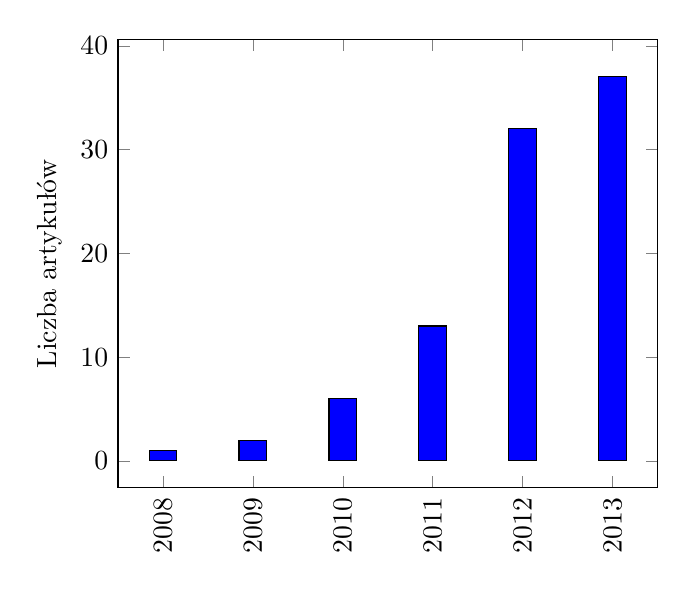
\begin{tikzpicture}
        \begin{axis}[
                bar width=10pt,
                %title=Liczba czasopism publikujących artykuły o Hadoop,
                % xlabel=Rok,
                ylabel=Liczba artykułów,
                symbolic x coords={2008, 2009, 2010, 2011, 2012, 2013},
                xtick=data,
                x tick label style={rotate=90, anchor=east}
            ]
            \addplot[ybar,fill=blue] coordinates {
                (2008,   1)
                (2009,   2)
                (2010,   6)
                (2011,   13)
                (2012,   32)
                (2013,   37)
            };
        \end{axis}
    \end{tikzpicture}
    \caption{Liczba czasopism publikujących artykuły o Hadoop}
    \label{fig:journal:hadoop}
\end{figure}

\begin{figure}
    \centering
    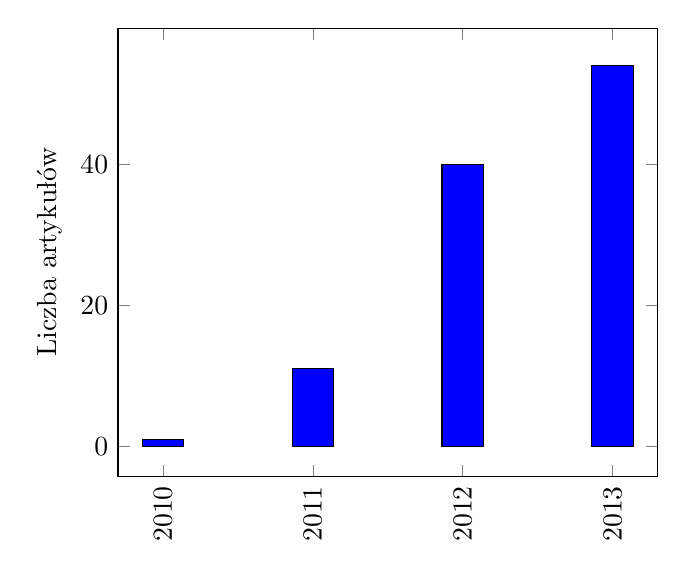
\begin{tikzpicture}
        \begin{axis}[
                bar width=15pt,
                %title=Liczba patentów dotyczących Hadoop,
                % xlabel=Rok,
                ylabel=Liczba artykułów,
                symbolic x coords={2010, 2011, 2012, 2013},
                xtick=data,
                x tick label style={rotate=90, anchor=east}
            ]
            \addplot[ybar,fill=blue] coordinates {
                (2010,	 1)
                (2011,   11)
                (2012,   40)
                (2013,   54)
            };
        \end{axis}
    \end{tikzpicture}
    \caption{Liczba patentów dotyczących Hadoop}
    \label{fig:patent:hadoop}
\end{figure}

\begin{figure}
    \centering
    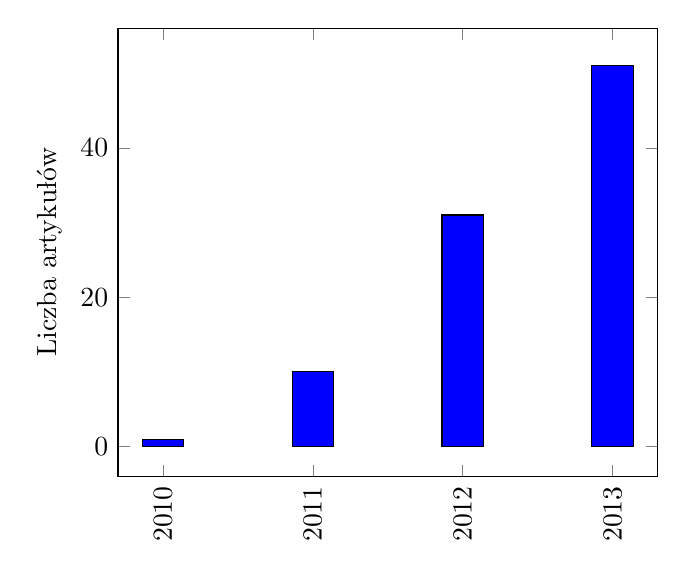
\begin{tikzpicture}
        \begin{axis}[
                bar width=15pt,
                %title=Liczba zgłaszających patenty związane z Hadoop,
                % xlabel=Rok,
                ylabel=Liczba artykułów,
                symbolic x coords={2010, 2011, 2012, 2013},
                xtick=data,
                x tick label style={rotate=90, anchor=east}
            ]
            \addplot[ybar,fill=blue] coordinates {
                (2010,	 1)
                (2011,   10)
                (2012,   31)
                (2013,   51)
            };
        \end{axis}
    \end{tikzpicture}
    \caption{Liczba zgłaszających patenty związane z Hadoop}
    \label{fig:invent:hadoop}
\end{figure}

\begin{figure}
    \centering
    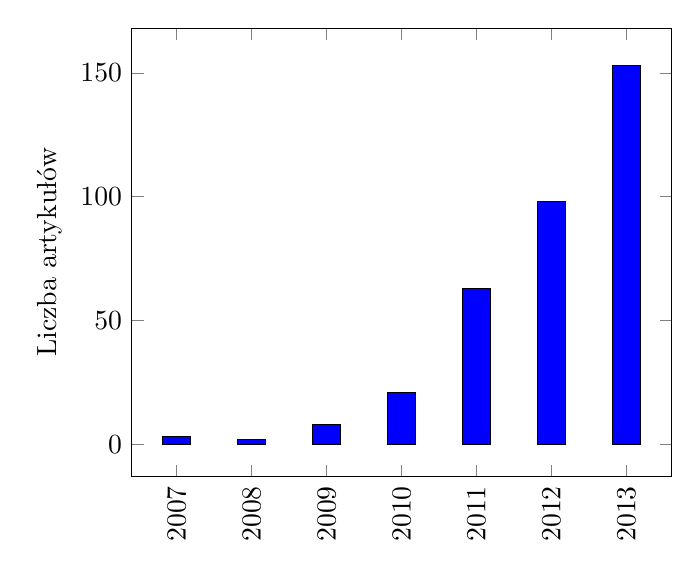
\begin{tikzpicture}
        \begin{axis}[
                bar width=10pt,
                %title=Liczba artykułów dotyczących MapReduce,
                % xlabel=Rok,
                ylabel=Liczba artykułów,
                symbolic x coords={2007, 2008, 2009, 2010, 2011, 2012, 2013},
                xtick=data,
                x tick label style={rotate=90, anchor=east}
            ]
            \addplot[ybar,fill=blue] coordinates {
                (2007,	 3)
                (2008,   2)
                (2009,   8)
                (2010,   21)
                (2011,   63)
                (2012,   98)
                (2013,   153)
            };
        \end{axis}
    \end{tikzpicture}
    \caption{Liczba artykułów dotyczących MapReduce}
    \label{fig:art:mapreduce}
\end{figure}

\begin{figure}
    \centering
    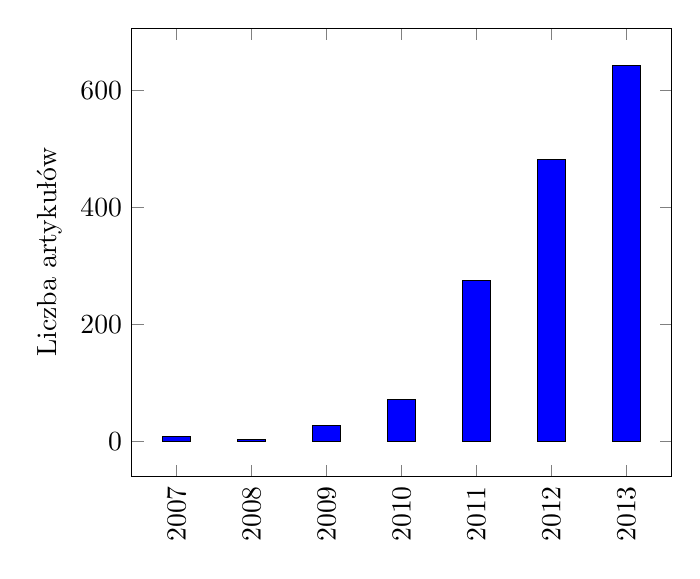
\begin{tikzpicture}
        \begin{axis}[
                bar width=10pt,
                %title=Liczba autorów piszących o MapReduce,
                % xlabel=Rok,
                ylabel=Liczba artykułów,
                symbolic x coords={2007, 2008, 2009, 2010, 2011, 2012, 2013},
                xtick=data,
                x tick label style={rotate=90, anchor=east}
            ]
            \addplot[ybar,fill=blue] coordinates {
                (2007,	 8)
                (2008,   4)
                (2009,   28)
                (2010,   72)
                (2011,   275)
                (2012,   482)
                (2013,   642)
            };
        \end{axis}
    \end{tikzpicture}
    \caption{Liczba autorów piszących o MapReduce}
    \label{fig:aut:mapreduce}
\end{figure}

\begin{figure}
    \centering
    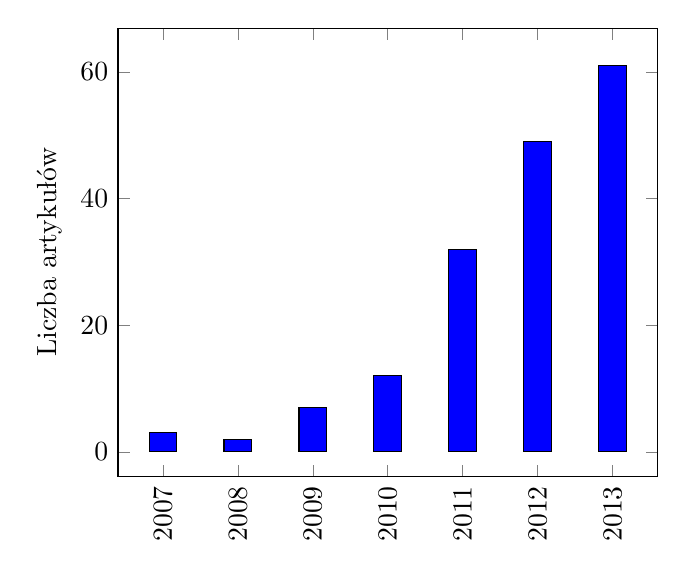
\begin{tikzpicture}
        \begin{axis}[
                bar width=10pt,
                %title=Liczba czasopism publikujących artykuły o MapReduce,
                % xlabel=Rok,
                ylabel=Liczba artykułów,
                symbolic x coords={2007, 2008, 2009, 2010, 2011, 2012, 2013},
                xtick=data,
                x tick label style={rotate=90, anchor=east}
            ]
            \addplot[ybar,fill=blue] coordinates {
                (2007,	 3)
                (2008,   2)
                (2009,   7)
                (2010,   12)
                (2011,   32)
                (2012,   49)
                (2013,   61)
            };
        \end{axis}
    \end{tikzpicture}
    \caption{Liczba czasopism publikujących artykuły o MapReduce}
    \label{fig:journal:mapreduce}
\end{figure}

\begin{figure}
    \centering
    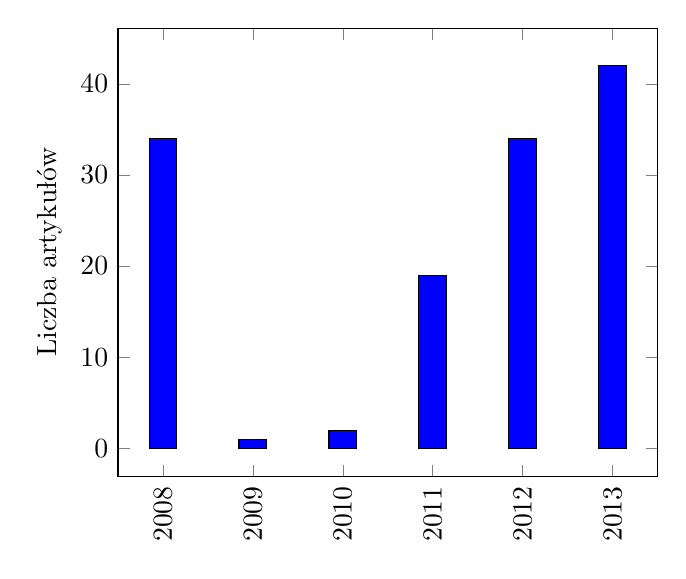
\begin{tikzpicture}
        \begin{axis}[
                bar width=10pt,
                %title=Liczba patentów dotyczących MapReduce,
                % xlabel=Rok,
                ylabel=Liczba artykułów,
                symbolic x coords={2008, 2009, 2010, 2011, 2012, 2013},
                xtick=data,
                x tick label style={rotate=90, anchor=east}
            ]
            \addplot[ybar,fill=blue] coordinates {
                (2008,   34)
                (2009,   1)
                (2010,   2)
                (2011,   19)
                (2012,   34)
                (2013,   42)
            };
        \end{axis}
    \end{tikzpicture}
    \caption{Liczba patentów dotyczących MapReduce}
    \label{fig:patent:mapreduce}
\end{figure}

\begin{figure}
    \centering
    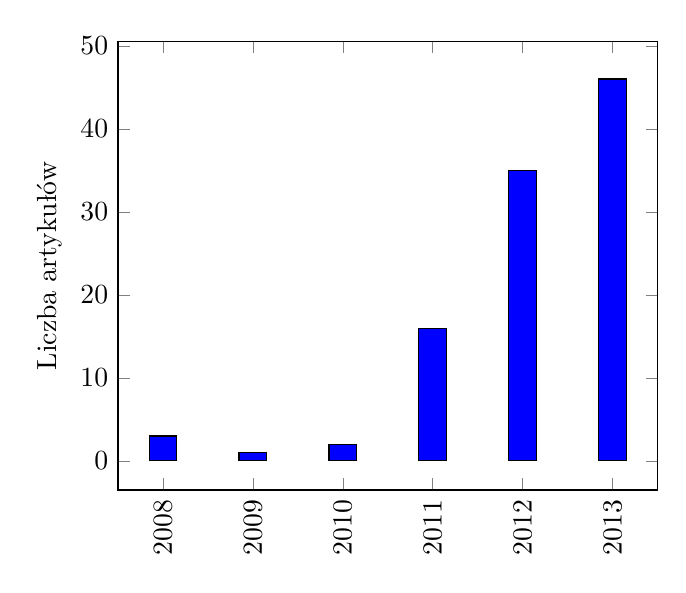
\begin{tikzpicture}
        \begin{axis}[
                bar width=10pt,
                %title=Liczba zgłaszających patenty związane z MapReduce,
                % xlabel=Rok,
                ylabel=Liczba artykułów,
                symbolic x coords={2008, 2009, 2010, 2011, 2012, 2013},
                xtick=data,
                x tick label style={rotate=90, anchor=east}
            ]
            \addplot[ybar,fill=blue] coordinates {
                (2008,   3)
                (2009,   1)
                (2010,   2)
                (2011,   16)
                (2012,   35)
                (2013,   46)
            };
        \end{axis}
    \end{tikzpicture}
    \caption{Liczba zgłaszających patenty związane z MapReduce}
    \label{fig:invent:mapreduce}
\end{figure}

\begin{table}[t]
    \centering
    \caption{Najczęściej występujące słowa kluczowe w artykułach o Big Data}
    \label{tabela_bigdata}
    \begin{tabular}{|c|c|}
        \hline 
        Słowo kluczowe & Liczba artykułów\\
        \hline
        big five & 83 \\
        \hline
        data mining & 56 \\
        \hline
        personality & 47 \\
        \hline
        classification & 21 \\
        \hline
        general factor of personality & 19 \\
        \hline
        endothelin & 18 \\
        \hline
        bioinformatics & 16 \\
        \hline
        clustering & 16 \\
        \hline
        data warehouse & 16 \\
        \hline
        database & 16 \\
        \hline
        big endothelin-1 & 15 \\
        \hline
        big data & 14 \\
        \hline
        endothelin-1 & 14 \\
        \hline
        data acquisition & 13 \\
        \hline
        data protection & 13 \\
        \hline
        privacy & 12 \\
        \hline
        cloud computing & 11 \\
        \hline
        cluster analysis & 11 \\
        \hline
        data sharing & 11 \\
        \hline
        gis & 11 \\
        \hline
        data analysis & 10 \\
        \hline
        data management & 10 \\
        \hline
        databases & 10 \\
        \hline
        internet & 10 \\
        \hline
    \end{tabular}
\end{table}

\begin{table}[t]
    \centering
    \caption{Najczęściej występujące słowa kluczowe w artykułach o Hadoop}
    \label{tabela_hadoop}
    \begin{tabular}{|c|c|}
        \hline 
        Słowo kluczowe & Liczba artykułów\\
        \hline
        cloud computing & 54 \\
        \hline
        mapreduce & 40 \\
        \hline
        hadoop & 20 \\
        \hline
        distributed computing & 10 \\
        \hline
    \end{tabular}
\end{table}

\begin{table}[t]
    \centering
    \caption{Najczęściej występujące słowa kluczowe w artykułach o MapReduce}
    \label{tabela_mapreduce}
    \begin{tabular}{|c|c|}
        \hline 
        Słowo kluczowe & Liczba artykułów\\
        \hline
        cloud computing & 64 \\
        \hline
        mapreduce & 62 \\
        \hline
        hadoop & 18 \\
        \hline
        scheduling & 11 \\
        \hline
        distributed computing & 10 \\
        \hline
    \end{tabular}
\end{table}

% section Analiza literatury (end)
